\chapter{Work Done}
We started out by trying to find a good application to instrument using Tracing Plane abstractions and investigated a couple of distributed concurrent programming frameworks, namely Akka and Finagle. But we soon realized that a typical distributed system used in production is built using a lot of different components and focusing on homogeneous framworks such as Finagle will not reveal the intricacies that we would like to learn about in instrumenting using tracing plane. We ultimately decided on OpenWhisk as it both seemed like a typical distributed system and seemed well supported by the community.

\section{Apache OpenWhisk}
\begin{figure}[htb]
\centering
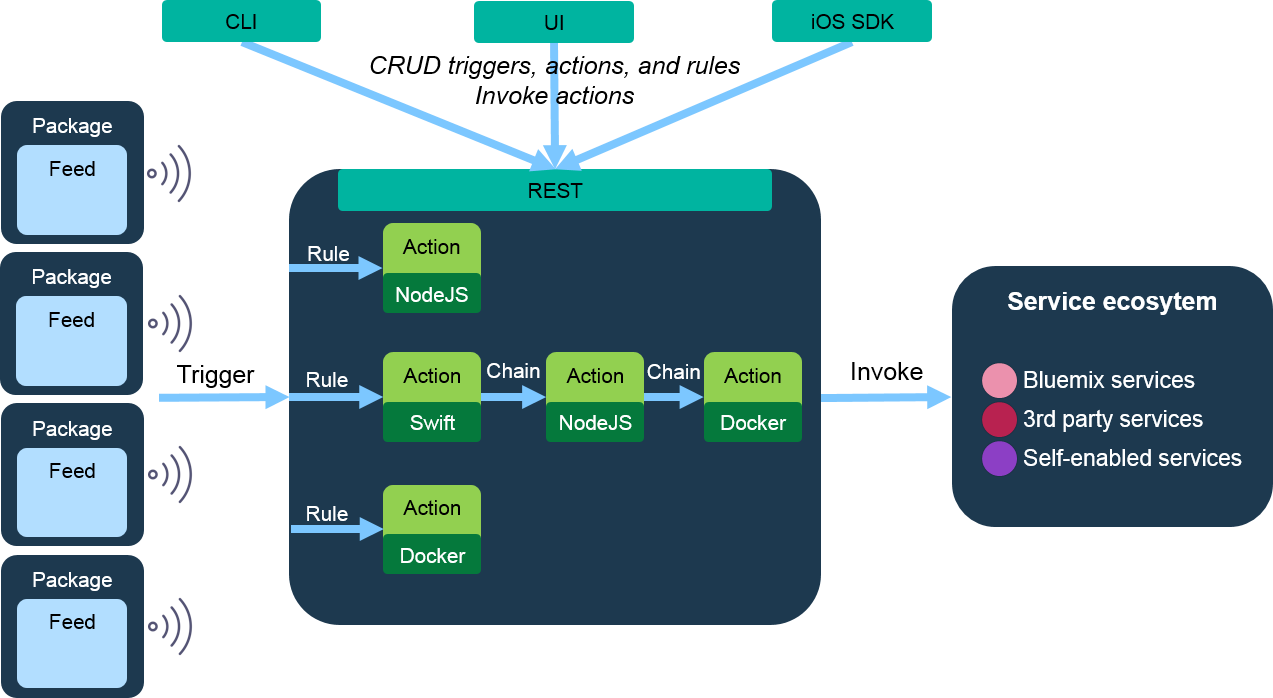
\includegraphics[scale=0.6]{./OpenWhisk}
\caption{OpenWhisk Architecture}
\label{fig:owarch}
\end{figure}
OpenWhisk is a serverless/FaaS platform which executes code in response to events. It supports synchronous, asynchronous and periodic invocation models using an event-driven programming model. Figure \ref{fig:owarch} shows its architecture. Basically, users can store functions or actions in the system that get triggered based on user-specified rules on either periodic events such as alarms or through the exposed REST API from a CLI.

\begin{figure}[htb]
\centering
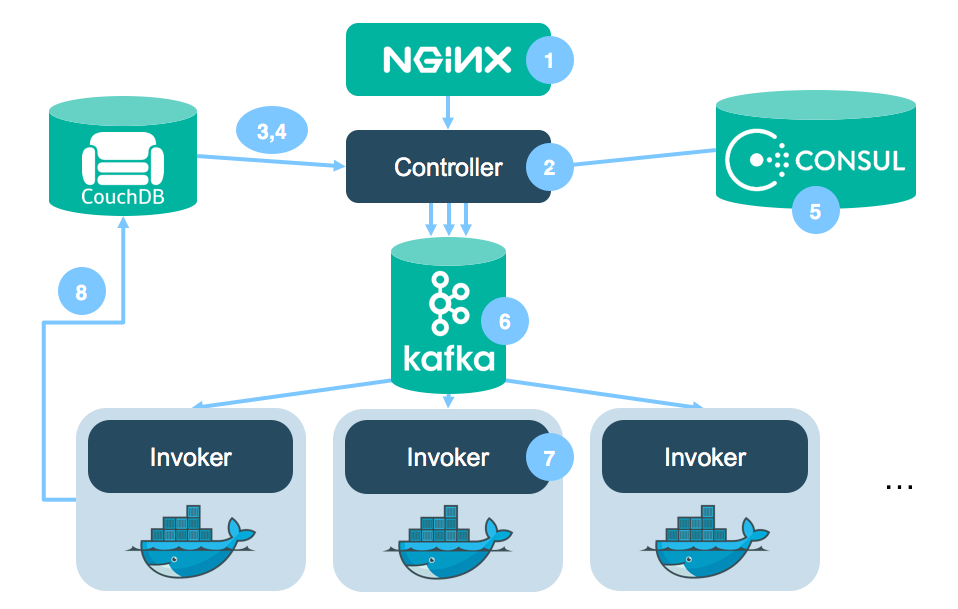
\includegraphics[scale=0.4]{./OpenWhisk_flow_of_processing}
\caption{Internal flow of processing in OpenWhisk}
\label{fig:owflow}
\end{figure}

Figure \ref{fig:owflow} shows what happens inside OpenWhisk during request processing. The system consists of nginx (written in C) for handling HTTP API requests, CouchDB (Erlang) for persistence, Consul (Go) for service discovery, Kafka (Scala, Java) for message queuing (these are all off-the-shelf third-party components), and two custom components written in Scala: a Controller and an Invoker.

When an HTTP request to process an action comes to the system, it is passed by nginx to the Controller (1, 2), which then talks to CouchDB to confirm whether the request can be authenticated and authorized (3). The Controller then retrieves the action associated with the request also stored in CouchDB (4) and then consults Consul to find out which Invoker (executor) is available (5). The Controller then queues the request in Kafka (6) which returns an \emph{ActivationId} that can be returned to the user (in case of an asynchronous request). The Invokers live in sandboxed Docker containers and execute (invoke) the action associated with the request (7). The result is then store in CouchDB (8) to be later retrieved by the user using a similar HTTP request.

\section{Challenges}

The challenges involved in instrumenting such a system are pretty much the same as those described earlier in section \ref{sec:challenge}.

Specifically, we are working on implementing opaque baggage contexts provided by the tracing plane in each component of OpenWhisk: Controller, Invoker, Nginx, CouchDB, Consul and Kafka. It is relatively easy to do that for the Controller and Invoker as both of them are written in Scala and relatively small code bases. Kafka, also written in Scala/Java, should also be easier. But for other components, written in non-JVM languages: C, Erlang and Go, we are limited by the current implementation of Tracing Plane which only supports JVM languages.

An additional challenge is investigating how should invokation models such as asynchronous and periodic requests be supported and exposed to the end user.

\section{Current Status}
We have started out by focusing on the Controller and Invoker which are core parts of OpenWhisk system and the easiest to instrument (among other components). This is reasonable because we can consider serializing and deserializing our baggage contexts into JSON and HTTP headers as part of the usual interactions across system boundaries which should still give us a good picture.

We have successfully integrated\cite{web:instru} Brown Tracing Framework's\cite{web:btf} X-Trace logging on the top of OpenWhisk's custom logging implementation which gives us an initial but partial view of the flow of a client request being processed by OpenWhisk. We are currently in process of integrating more pervasive logging with the help of X-Trace's automatic instrumentation libraries (which are based on AspectJ aspects), which can automatically propagate baggage with each use of Scala's Futures and Promises. This should give us a lot more visibility into the operations of the Controller and the Invokers as they process a request. However, much of the hard work of making rest of the system components interoperate with our baggage remains.
